\normalfalse \difficilefalse \tdifficiletrue
\correctionfalse

%\UPSTIidClasse{11} % 11 sup, 12 spé
%\newcommand{\UPSTIidClasse}{12}

\exer{Maxpid $\star\star\star$ \label{B2:12:18}}
\setcounter{numques}{0}
\UPSTIcompetence{B2-12}
\index{Compétence B2-12}
\index{Maxpid}
\ifcorrection
\else
\textbf{Pas de corrigé pour cet exercice.}
\fi

\ifprof
\else

Soit le schéma suivant. 
\begin{center}
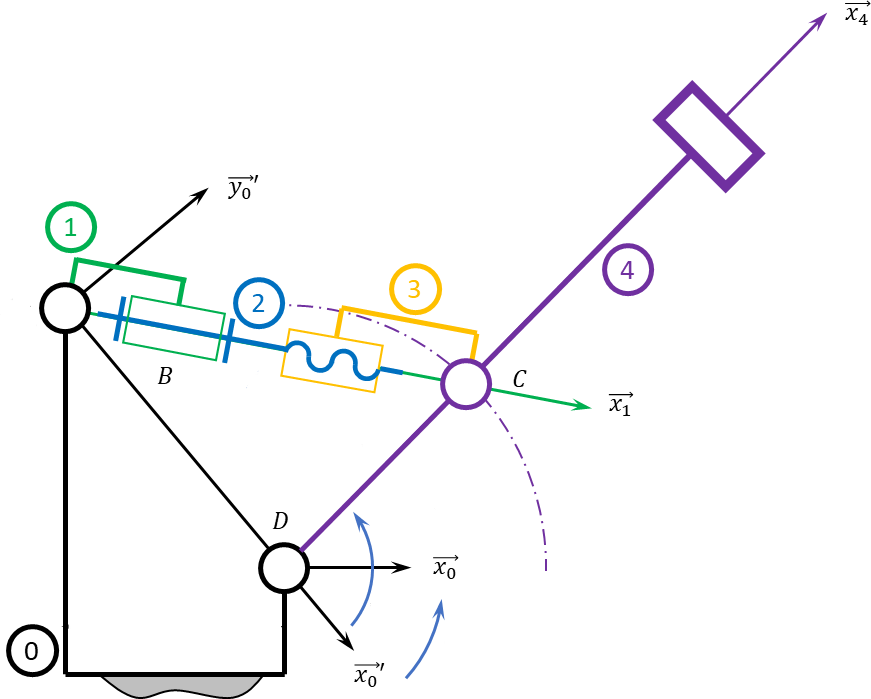
\includegraphics[width=\linewidth]{18_01}
\end{center}
\fi

Par ailleurs $a=\SI{107,1}{mm}$, $b=\SI{80}{mm}$, $c=\SI{70}{mm}$, $d=\SI{80}{mm}$. Le pas de la vis est de $\SI{4}{mm}$.


\question{Tracer le graphe des liaisons.}
\ifprof
\else
\fi

\question{Retracer le schéma cinématique pour $\theta(t)=0\,\text{rad}$.}
\ifprof
\else
\fi

\question{Retracer le schéma cinématique pour $\theta(t)=\dfrac{\pi}{2}\,\text{rad}$.}
\ifprof
\else
\fi


\question{En déduire la course de $\lambda$.}
\ifprof
\else
\fi



\ifprof
\else
\begin{flushright}
\footnotesize{Corrigé  voir \ref{B2:12:18}.}
\end{flushright}%
\fi